


\documentclass[12pt]{article}

%\usepackage[pass,showframe]{geometry}% just to show the page margins
\usepackage{graphicx}% remove demo option in the actual document
%\graphicspath{{images/}} %configuring the graphicx package
\begin{document}
%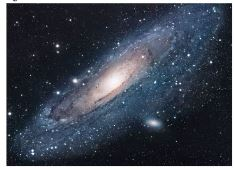
\includegraphics{images/1.JPG}
this is my figure \ref{fig:FebAA_Working} and \ref{FebAA_Working}. 

\begin{figure}
\caption{This is our caption }
  %\centering
    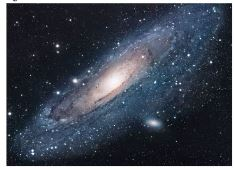
\includegraphics[width=10cm, height=5cm]{images/1}
    
\label{fig:FebAA_Working}       % Give a unique label
\end{figure}









In figure \ref{FebAA_Working} we have explained etc.... 



The universe is immense and it seems to be homogeneous, 
on a large scale, everywhere we look.

\begin{figure}
  \centering
    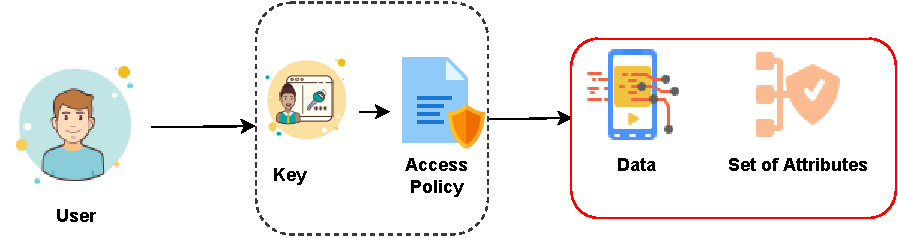
\includegraphics[width=10cm, height=5cm]{images/2.333.pdf}
    \caption{This is our caption }
\label{FebAA_Working}       % Give a unique label
\end{figure}





% The \includegraphcs command is 
% provided (implemented) by the 
% graphicx package
  
 
There's a picture of a galaxy above.

























\section{Method 2}
this is our figure \ref{fig:2.14}
\begin{figure}[h]
  \centering
  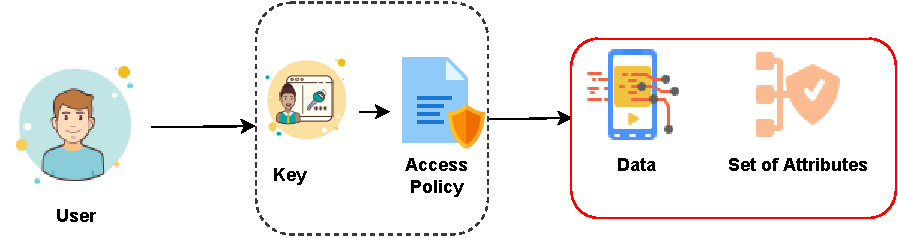
\includegraphics[width=0.5\textwidth,height=3.5cm]{images/2.333.pdf}
  \caption{geometry. This is our figure}
  \label{fig:2.14}

\end{figure}



\end{document}

[h]: Place the figure "here" at the approximate location in the text where the figure command is declared. However, if there is not enough space on the current page, LaTeX may still move the figure to the top or bottom of the page.

[t]: Place the figure at the top of a page.

[b]: Place the figure at the bottom of a page.

Figure file types
make sure the figures have same type, it is allowed in latex but you may have problem while submitting the paper. 